\section{Base de datos de señales de habla y ruido}
\label{sec:audio_db}

Para poder entrenar, comparar y evaluar los algoritmos de supresión de ruido es necesario contar con una base de datos de señales de habla y otra de ruidos. Contando con ambas bases es posible generar una base de datos de señales de habla ruidosa que se utilizarán como la señal de entrada a los filtros.

La base de datos utilizada fue la descrita en el trabajo \emph{A scalable noisy speech dataset and online subjective test framework} \cite{a_scalable_noisy_speech_dataset_and_online_subjective_test_framework}.

\subsection{Señales de entrenamiento y de pruebas}

La base de datos se encuentra dividida dos conjuntos disjuntos:

\begin{itemize}
	\item Conjunto de entrenamiento: El filtro basado en redes neuronales depende de un conjunto de entrenamiento que se encarga de optimizar los parámetros de la red de tal manera que el error sea el menor posible. El filtro adaptativo no requiere de un conjunto de entrenamiento ya que sus parámetros son optimizados en tiempo real.
	\item Conjunto de prueba: Para evaluar cada filtro de manera objetiva, se utiliza el conjunto de pruebas.
\end{itemize}

\subsection{Señales de habla sin ruido}

La base de señales de habla sin ruido esta dividida en los conjuntos de entrenamiento y de prueba. El conjunto de entrenamiento consiste en más de 20.000 oraciones leídas en voz alta por 56 oradores, 28 masculinos y 28 femeninos. Las oraciones tienen una duración media de aproximadamente 3 segundos y se encuentran muestreadas a 16 kHz. Las oraciones consisten en extractos del diario \emph{Scottish Herald}.

El conjunto de pruebas esta formado por mas de 1.000 oraciones leídas por 20 oradores femeninos y masculinos. Las oraciones tienen una duración media de aproximadamente 12 segundos y se encuentran muestreadas a 16 KHz. Las oraciones pertenecen a la base descrita en el trabajo \emph{A Pitch Tracking Corpus with Evaluation on Multipitch Tracking Scenario} \cite{a_pitch_tracking_corpus_with_evaluation_on_multipitch_tracking_scenario}.

\subsection{Señales de ruido}

La base de señales de ruido, también esta dividida en los conjuntos de entrenamiento y de prueba. Los ruidos fueron seleccionados de la base descrita en el trabajo \emph{DEMAND: a collection of multi-channel recordings of acoustic noise in diverse environments} \cite{demand_a_collection_of_multi_channel_recordings_of_acoustic_noise_in_diverse_environments}, y de \emph{freesound.org}.

Las señales de ruido consisten en 14 tipos de ruidos: aire acondicionado, anuncios por alto parlante, autos, impresora, puertas, masticar, personas hablando, vecinos hablando, sillas, tráfico, calles y avenidas, tipeo y aspiradora.

Al igual que las señales de habla, todas las señales de ruido fueron muestreadas a 16 kHz.

\subsection{Generación de señales de habla ruidosas}
\label{sec:noisy_signals_generation}

Como dijimos al comienzo de la presente sección, a partir de la base de señales de habla y de la base de señales de ruidos, es posible generar la base de señales de habla ruidosa. 

Los algoritmos se desempeñarán de manera diferente dependiendo del nivel de ruido ($SNR$) que tenga cada una de las señales procesadas. El presente trabajo se limita a trabajar con el siguiente conjunto de niveles $SNR$:

\begin{equation*}
	\{ \SI{-5}{dB}, \; \SI{0}{dB}, \; \SI{5}{dB}, \; \SI{10}{dB}, \; \SI{15}{dB}, \; \SI{20}{dB} \}
\end{equation*}

\subsubsection{Mezclado de señales}

El primer paso para mezclar la señal de habla con la señal de ruido es normalizar ambas señales de tal manera que tengan el mismo valor RMS. A este proceso se le llama normalización RMS.

Dada una señal de habla $s[k]$ y una señal de ruido $n[k]$, supongamos que se quiere hallar $c_1$ tal que la señal $c_1 \; s[k]$ tenga cierto valor $RMS$ igual a $b$, es decir:

\begin{equation*}
	RMS\{c_1 \; s[k]\} = b
\end{equation*}

El valor RMS de la señal escalada viene dado por:

\begin{equation*}
	b = \sqrt{\frac{1}{K} \sum_{\forall k} (c_1 \; s[k])^2}
\end{equation*}

\noindent entonces:

\begin{equation*}
	c_1 = \sqrt{\frac{K \; b^2}{\sum_{\forall k} s[k]^2}} = \frac{b}{RMS\{s[k]\}}
\end{equation*}

El valor RMS escogido fue de $\SI{-25}{dB}$, entonces el factor $c$ se obtiene como:

\begin{equation*}
	c_1 = \frac{10^{\frac{-25}{20}}}{RMS\{s[k]\}}
\end{equation*}

Finalmente obtenemos:

\begin{equation*}
	s'[k] = \frac{10^{\frac{-25}{20}}}{RMS\{s[k]\}} \; s[k] \qquad \text{y} \qquad n'[k] = \frac{10^{\frac{-25}{20}}}{RMS\{s[k]\}} \; n[k]
\end{equation*}

El segundo paso es mezclar ambas señales a un determinado valor de $SNR$. Para ello debemos calcular el factor de escalado $c_2$, a aplicar en la señal de ruido, tal que:

\begin{equation*}
	SNR = \frac{RMS\{s'[k]\}}{RMS\{c_2 \; n'[k]\}}
\end{equation*}

\noindent entonces:

\begin{equation*}
	c_2 = \frac{RMS\{s'[k]\}}{SNR \quad RMS\{n'[k]\}}
\end{equation*}

\noindent y dado que usualmente el valor $SNR$ es expresado en $\si{dB}$ tenemos que:

\begin{equation*}
	c_2 = \frac{RMS\{s'[k]\}}{10^{\frac{SNR}{20}} \quad RMS\{n'[k]\}}
\end{equation*}

Luego se obtiene la señal de habla ruidosa calculando:

\begin{equation*}
	y'[k] = s'[k] + c_2 \; n'[k]
\end{equation*}

Por último es necesario contar con señales de habla ruidosas con distintas intensidades, por este motivo se realizó una nueva normalización RMS con un valor objetivo aleatorio de entre $\SI{-15}{dB}$ y $\SI{-35}{dB}$. Dado $l$ el valor RMS aleatorio en decibeles, el factor de escalado se calcula como:

\begin{equation*}
	c_3 = \frac{10^{\frac{l}{20}}}{RMS\{y[k]\}}
\end{equation*}

Finalmente la señal de habla ruidosa viene dada por:

\begin{equation*}
	y[k] = c_3 \left( s'[k] + c_2 \; n'[k] \right)
\end{equation*}

\subsubsection{Base de señales de habla ruidosa}

A partir de el conjunto de entrenamiento de señales de habla sin ruido y del conjunto de entrenamiento de señales de ruido, utilizando el proceso de mezclado descrito en la sección anterior, se generó el conjunto de entrenamiento de señales de habla ruidosa. Lo mismo se realizó para generar el conjunto de pruebas de señales de habla ruidosa. A continuación se detallan los pasos realizados:

\begin{itemize}
	\item Se escoge aleatoriamente un señal de habla sin ruido.
	\item Se escoge una señal de ruido.
	\item En el paso anterior, pueden suceder dos cosas, que el ruido escogido tenga mayor o menor duración que la señal de habla. En el caso que tenga menor, se escoge otra señal de ruido, repitiendo este proceso hasta llegar a la duración de la señal de habla.
	\item Se mezclan ambas señales utilizando un nivel de SNR aleatorio en el conjunto \{-5, 0, 5, 10, 15, 20, 40\}.
	\item Cada señal de habla es al menos utilizada dos veces y mezclada con ruidos distintos.
	\item El proceso se repite hasta utilizar todas las señales de habla. Las señales de ruido son reutilizadas hasta cubrir el total de señales de habla.
\end{itemize}

El conjunto de entrenamiento resultante consta de aproximadamente 38 horas de duración y el conjunto de pruebas resultante de 7 horas.


\subsection{Niveles base de PESQ y STOI}

Cada señal de habla ruidosa tendrá cierto nivel base para las medidas PESQ y STOI. El objetivo de los algoritmos de supresión de ruido es mejorar el nivel base.

Dependiendo de las características de cada señal ruidosa, el nivel base será diferente.

Las figuras \ref{fig:ch5_pesq_histogram} y \ref{fig:ch5_stoi_histogram} muestran un histograma de los niveles base para los distintos valores de SNR utilizados.

\begin{figure}[H]
	\centering
	\centerline{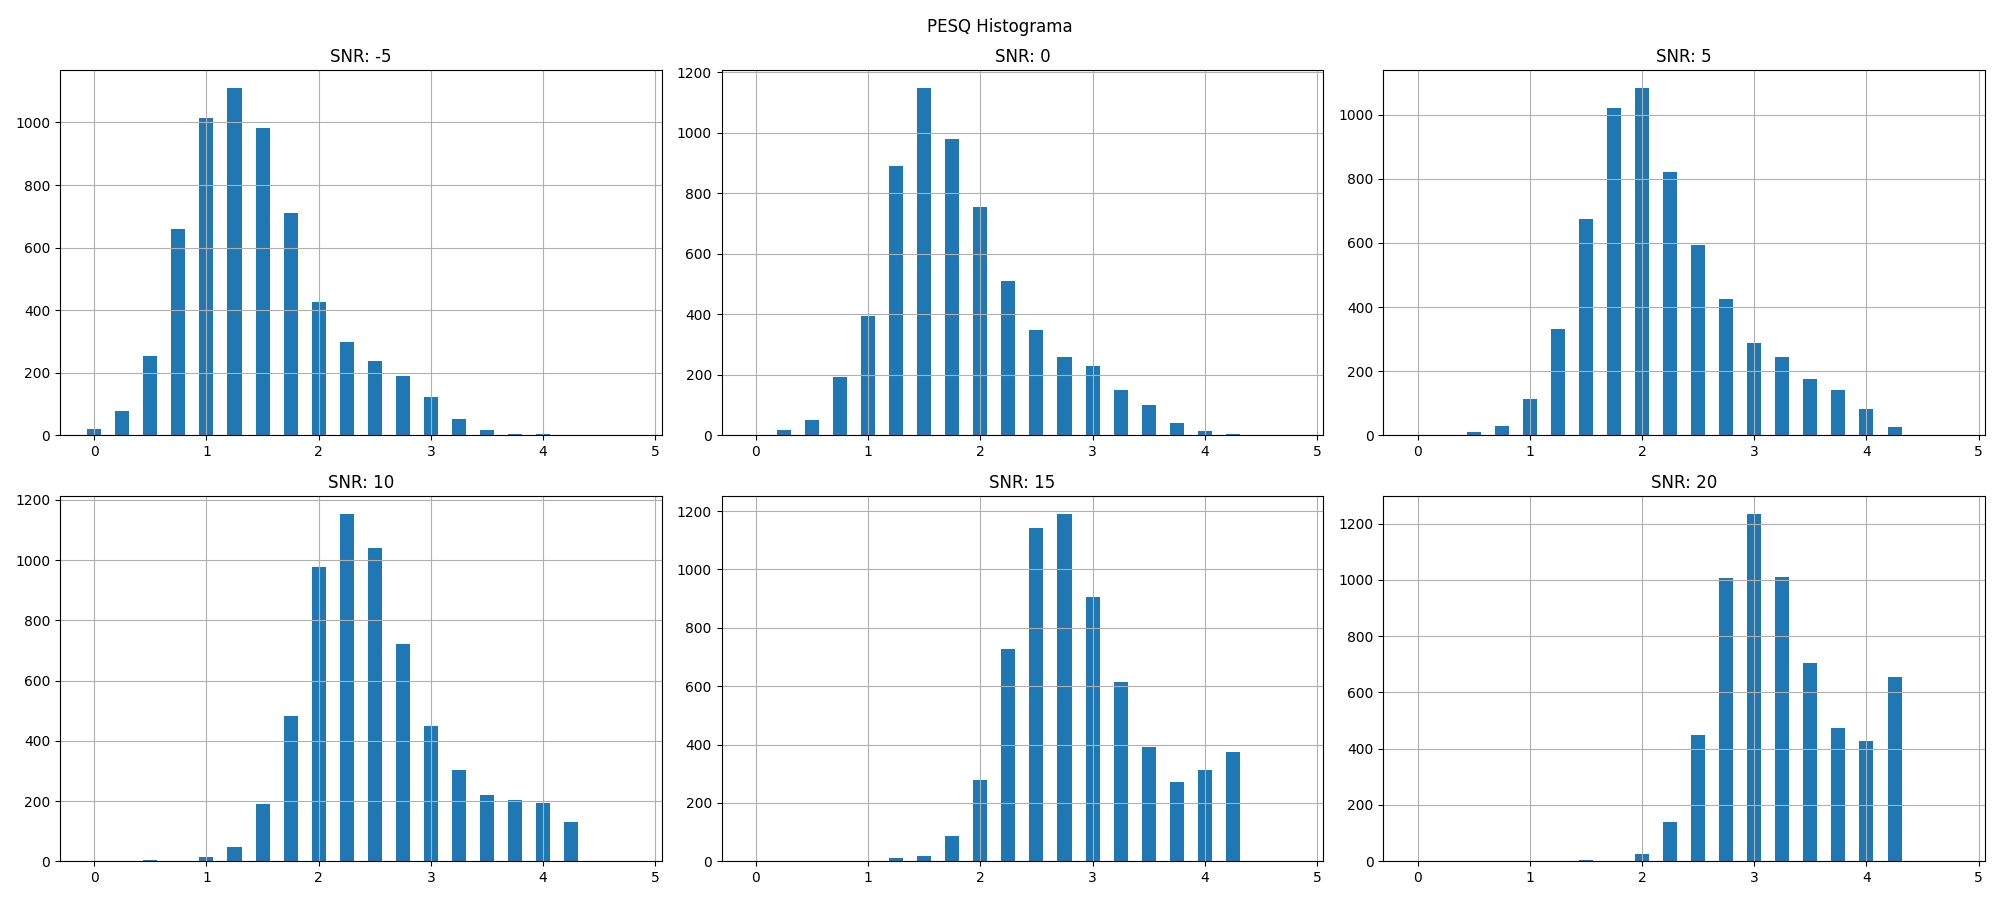
\includegraphics[scale=0.35]{images/ch5/pesq_aggregated.png}}
	\caption{Histograma PESQ.}
	\label{fig:ch5_pesq_histogram}
\end{figure}

\begin{figure}[H]
	\centering
	\centerline{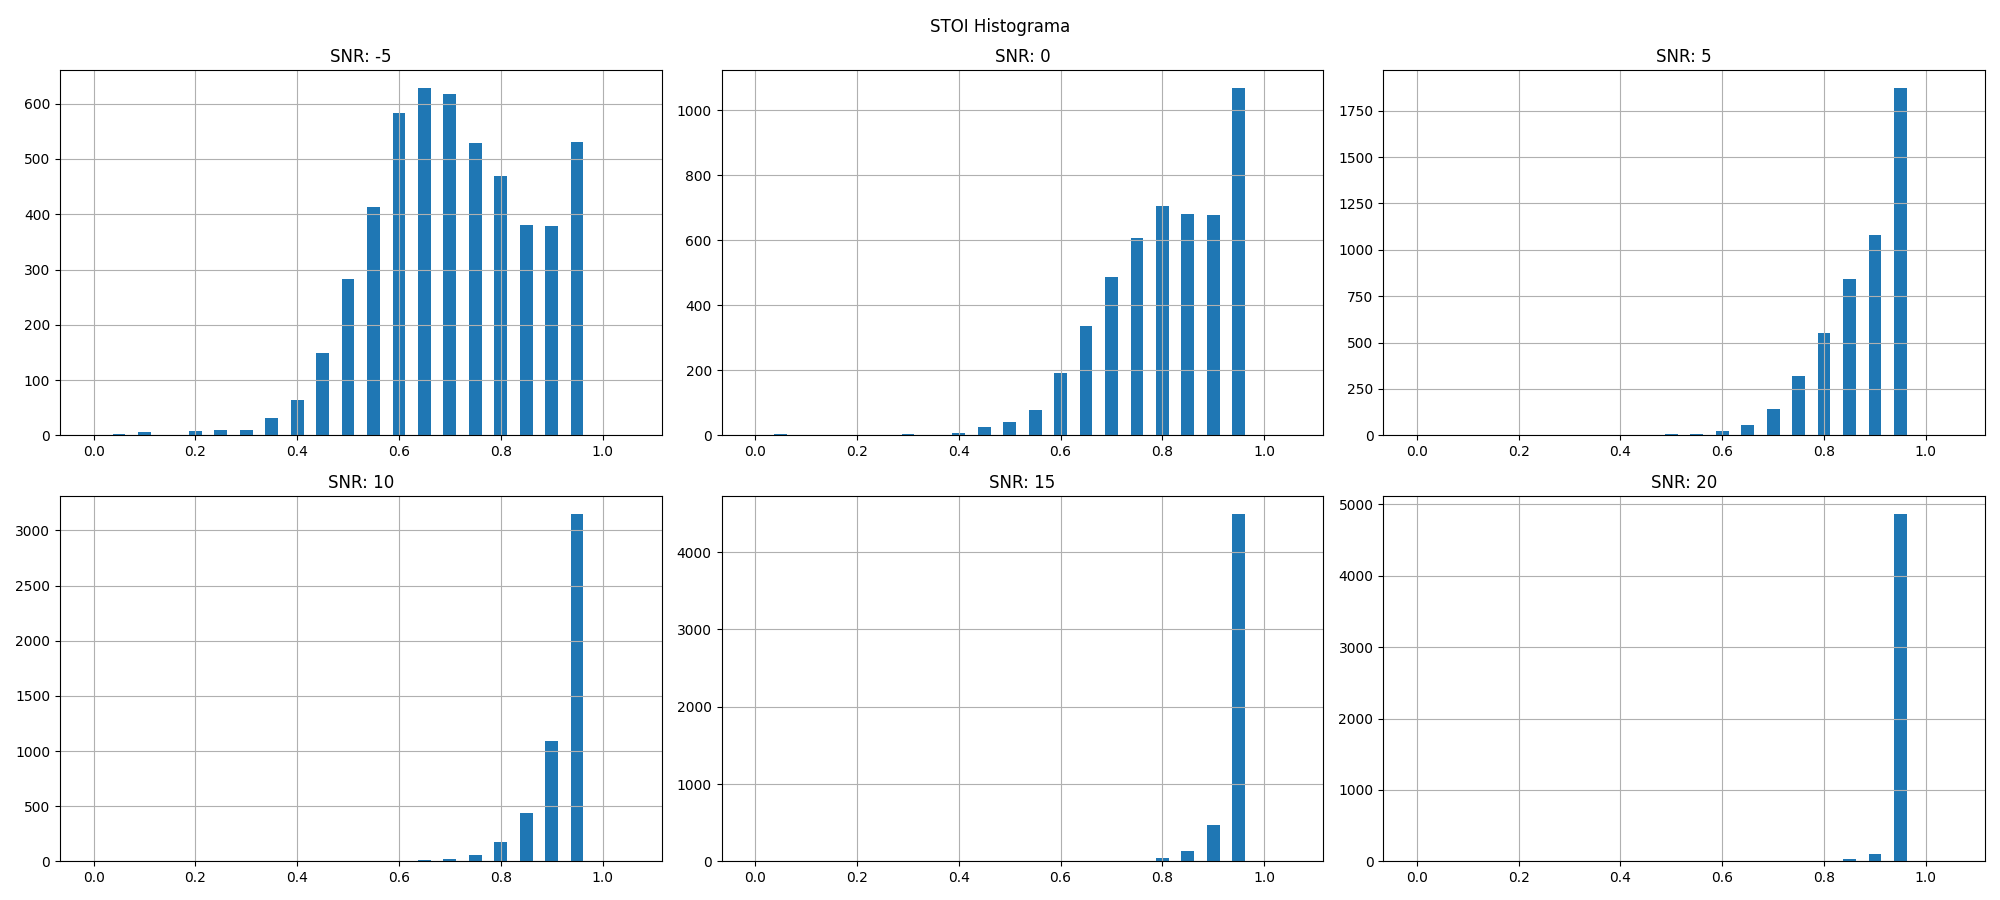
\includegraphics[scale=0.35]{images/ch5/stoi_aggregated.png}}
	\caption{Histograma STOI.}
	\label{fig:ch5_stoi_histogram}
\end{figure}

A medida que la SNR aumenta, los valores medio de PESQ y STOI se corren hacia la derecha, es decir se acercan al valor máximo, que para PESQ es de 4.5 y para STOI es de 1.

\subsection{Ruido correlacionado}

Como vimos en la sección \ref{sec:adaptive_filter_architecture}, el filtro adaptativo depende de dos señales de entrada; la señal de habla ruidosa $d(n)$ y la señal de ruido correlacionado $u(n)$. 

En la sección anterior vimos cómo se construyeron las señales de habla ruidosa mezclando señales de habla con señales de ruido, las cuales fueron obtenidas de bases de datos comúnmente utilizadas en experimentos relacionados con el presente trabajo. Sin embargo, para el caso de ruido correlacionado, no fue posible encontrar una base de datos obtenida a partir de grabaciones reales. Por tal motivo se optó por fabricar la base a partir de la base de señales de ruido.

Para fabricar el ruido correlacionado lo que se hizo fue partir la señal de ruido en bloques de largo aleatorio en el conjunto \{16384, 32768, 65536\}. Luego, a cada bloque se le aplicó un filtro $A$, nuevamente, de largo aleatorio en el rango [8, 12] cuyos coeficientes también son aleatorios en el rango [0, 1].

En una configuración como la que vimos en la figura \ref{fig:ch3_af-se-setup}, en algunas ocasiones es posible que ocurra el fenómeno de diafonía donde parte de la señal de habla $s(n)$ se mezcla con el ruido de referencia $n_2(n)$. Para simular condiciones similares a las encontradas en la práctica, además de realizar la transformación aleatoria descrita en el párrafo anterior, a la señal obtenida se le sumó un porcentaje $a$ de la señal de habla $s(n)$ aleatorio en el rango [0, 5].

Resumiendo, la señal de ruido de referencia fue obtenida como:

\begin{equation*}
	n_2(n) = A(n) \circledast n_1(n) + a(n) \cdot s(n)
\end{equation*}

\noindent donde $A(n)$ son los filtros aleatorios y $a(n)$ son los coeficientes aleatorios de diafonía.